% comment out for student version
\ifdefined\Student\relax\else\def\Teacher{}\fi

\documentclass[12pt]{article}

\title{Activity 3: Hardware}
\author{Dr. Chris Mayfield}
\date{CS 101, Fall 2020}

%\ProvidesPackage{cspogil}

% fonts
\usepackage[utf8]{inputenc}
\usepackage[T1]{fontenc}
\usepackage{mathpazo}

% spacing
\usepackage[margin=2cm]{geometry}
\renewcommand{\arraystretch}{1.4}
\setlength{\parindent}{0pt}

% orphans and widows
\clubpenalty=10000
\widowpenalty=10000
\pagestyle{empty}

% figures and tables
\usepackage{graphicx}
\usepackage{multicol}
\usepackage{tabularx}
\usepackage{wrapfig}

% fixed-width columns
\usepackage{array}
\newcolumntype{L}[1]{>{\raggedright\let\newline\\\arraybackslash\hspace{0pt}}m{#1}}
\newcolumntype{C}[1]{>{\centering\let\newline\\\arraybackslash\hspace{0pt}}m{#1}}
\newcolumntype{R}[1]{>{\raggedleft\let\newline\\\arraybackslash\hspace{0pt}}m{#1}}

% include paths
\makeatletter
\def\input@path{{Models/}{../../Models/}}
\graphicspath{{Models/}{../../Models/}}
\makeatother

% colors
\usepackage[svgnames,table]{xcolor}
\definecolor{bgcolor}{HTML}{FAFAFA}
\definecolor{comment}{HTML}{007C00}
\definecolor{keyword}{HTML}{0000FF}
\definecolor{strings}{HTML}{B20000}

% table headers
\newcommand{\tr}{\bf\cellcolor{Yellow!10}}

% syntax highlighting
\usepackage{textcomp}
\usepackage{listings}
\lstset{
    basicstyle=\ttfamily\color{black},
    backgroundcolor=\color{bgcolor},
    numberstyle=\scriptsize\color{comment},
    commentstyle=\color{comment},
    keywordstyle=\color{keyword},
    stringstyle=\color{strings},
    columns=fullflexible,
    keepspaces=true,
    showlines=true,
    showstringspaces=false,
    upquote=true
}

% code environments
\newcommand{\java}[1]{\lstinline[language=java]{#1}}%[
\lstnewenvironment{javalst}{\lstset{language=java,backgroundcolor=}}{}
\lstnewenvironment{javabox}{\lstset{language=java,frame=single,numbers=left}\quote}{\endquote}

% PDF properties
\usepackage[pdftex]{hyperref}
\urlstyle{same}
\makeatletter
\hypersetup{
  pdftitle={\@title},
  pdfauthor={\@author},
  pdfsubject={\@date},
  pdfkeywords={},
  bookmarksopen=false,
  colorlinks=true,
  citecolor=black,
  filecolor=black,
  linkcolor=black,
  urlcolor=blue
}
\makeatother

% titles
\makeatletter
\renewcommand{\maketitle}{\begin{center}\LARGE\@title\end{center}}
\makeatother

% boxes [optional height]
\newcommand{\emptybox}[1][10em]{
\vspace{1em}
\begin{tabularx}{\linewidth}{|X|}
\hline\\[#1]\hline
\end{tabularx}}

% models
\newcommand{\model}[1]{\section{#1}\nopagebreak}
\renewcommand{\thesection}{Model~\arabic{section}}

% questions
\newcommand{\quest}[1]{\subsection*{Questions~ (#1)}}
\newcounter{question}
\newcommand{\Q}{\vspace{1em}\refstepcounter{question}\arabic{question}.~ }
\renewcommand{\thequestion}{\#\arabic{question}}

% sub-question lists
\usepackage{enumitem}
\setenumerate[1]{label=\alph*)}
\setlist{itemsep=1em,after=\vspace{1ex}}

% inline answers
\definecolor{answers}{HTML}{C0C0C0}
\newcommand{\ans}[1]{%
\ifdefined\Student
    \leavevmode\phantom{~~\textcolor{answers}{#1}}
\else
    ~~\textcolor{answers}{#1}
\fi}

% longer answers [optional height]
\newsavebox{\ansbox}
\newenvironment{answer}[1][4em]{
\nopagebreak
\begin{lrbox}{\ansbox}
\begin{minipage}[t][#1]{\linewidth}
\color{answers}
}{
\end{minipage}
\end{lrbox}
\ifdefined\Student
    \phantom{\usebox{\ansbox}}%
\else
    \usebox{\ansbox}%
\fi}


\begin{document}

\maketitle

Have you ever wondered what goes on inside your smartphone?
Not just how the apps run, but how the hardware actually works?
Last week you designed a simple circuit that adds two 4-bit numbers.
With enough time and energy, you could learn to build an entire computer!
But that's not the goal of this course, so we'll abstract those details.
For now, let's take a look at how computers store and process information.

\model{Computer Architecture}

Here is the 8-bit machine described in Appendix~C of Brookshear and Brylow (2015):

\begin{center}
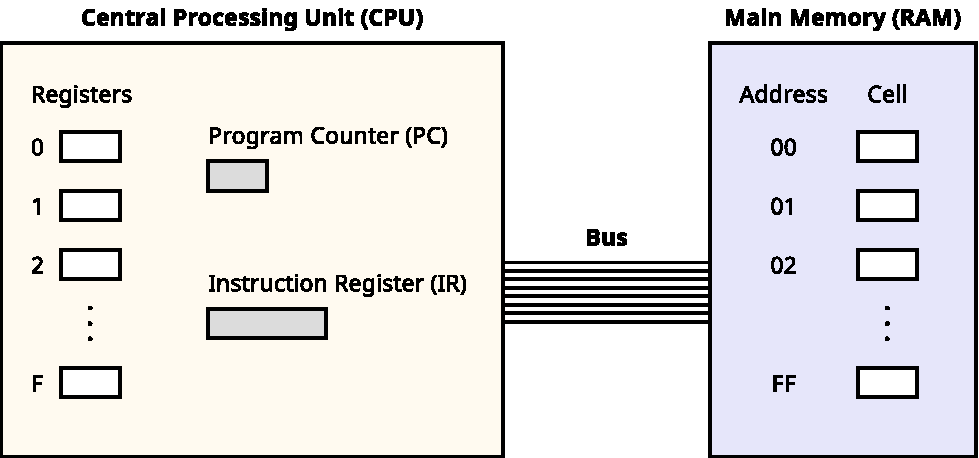
\includegraphics[width=0.8\linewidth]{cpu-bus-ram.pdf}
\end{center}


\quest{12 min}


\Q What are the three main components in the diagram?
Based on its name, what do you think each hardware component does?

\begin{answer}
The CPU is ``the brain'' of the computer that performs calculations and makes decisions.
The RAM is where ``working memory'' is stored.
The Bus connects the CPU and RAM together.
\end{answer}


\Q How many registers does the CPU have? How many memory cells are in RAM?
%Why do you think there are more memory cells than registers?

\begin{answer}[3em]
16 registers (0--F) and 256 memory cells (00--FF).
\end{answer}


\Q The CPU has circuits for adding the contents of two registers; think of registers as the ``pins'' in last week's lab.
What is the largest number this machine can add without overflowing?

\begin{answer}
Because the machine has eight bits, the largest number is 0xFF or 255.
\end{answer}


\Q Common tasks the CPU performs include \emph{loading} data from a memory cell into a register and \emph{storing} data from a register into a memory cell.
Describe what the CPU would need to do in order to add twenty numbers stored in memory.

\begin{answer}[7em]
The CPU would need to use two registers: one for a running total, and one to load data from memory.
Start by setting the total register to zero.
For each number, load it into the other register, and then add it to the total.
\end{answer}

\model{Machine Instructions}

%TODO replace images from textbook (Copyrighted by Pearson -- fair use?)

\begin{multicols}{2}
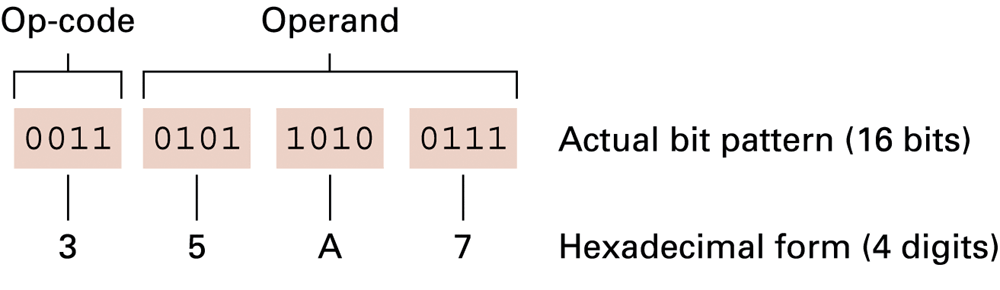
\includegraphics[width=\linewidth]{opcode1.png}

\columnbreak

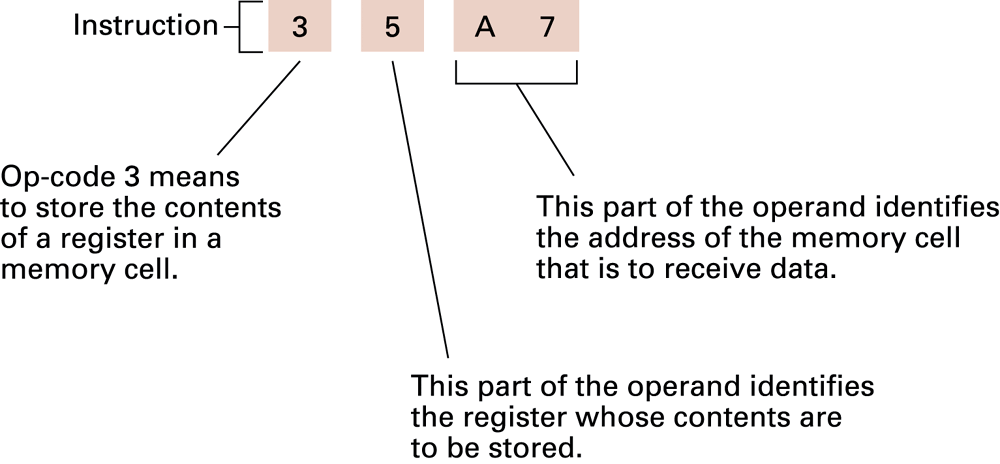
\includegraphics[width=\linewidth]{opcode2.png}
\end{multicols}


\quest{8 min}


\Q How many bits is the op-code? How many possible op-codes can the machine support?

\begin{answer}
With 4-bit op-codes, the machine can have at most 16 different op-codes.
\end{answer}


\Q The op-code for loading data from memory into a register is 1.
Write an instruction (in hex) for loading data from address 3D into register 4.

\begin{answer}[3em]
143D
\end{answer}


\Q Why is the instruction register in \ref{architecture.tex} twice as large as the other registers?
How many memory cells are needed to store a single instruction?

\begin{answer}
Instructions are 16 bits, and memory cells are 8 bits; one instruction takes up two cells.
Note the instructions need to be large enough for their operand to represent a memory address.
\end{answer}


\end{document}
